\documentclass[runningheads]{llncs}
%
\usepackage[T1]{fontenc}
\usepackage{graphicx}
\usepackage{amsmath}
\usepackage{url}
\usepackage{cite}
\usepackage{booktabs}
\usepackage{subcaption}

\begin{document}
%
\title{Three-Tier Embedded Variability Management for Mechatronic Product Lines: A Portable Integration Pattern in Digital LEGO}
%
\titlerunning{Three-Tier Embedded Variability in Digital LEGO}
%
\author{Aleksandra Erohina\inst{1} \and Christian Zehetner\inst{1} \and Georg Hackenberg\inst{1}}
%
\authorrunning{A. Erohina et al.}
%
\institute{University of Applied Sciences Upper Austria, Wels, Austria\\
\email{\{aleksandra.erohina, christian.zehetner, georg.hackenberg\}@fh-wels.at}}
%
\maketitle              % typeset the header of the contribution
%
\begin{abstract}
Managing variability in mechatronic systems requires a tight coupling between logical feature models and physical geometric assets. However, a significant "Agile Infrastructure Gap" exists between lightweight early-phase design and heavy industrial Product Lifecycle Management (PLM) solutions. This paper presents a novel three-tier architectural pattern for embedding variability management directly into the solution space using the open LDraw file format. By enforcing a formal separation between Configurations (Product Map), Features (Variability Logic), and Parts (Atomic Asset Base) within a single file, we enable a self-contained 150\% model. This approach utilizes a structured naming convention and hierarchical references to encode configuration rules, ensuring maximum portability across CAD editors without proprietary plugins. We validate the pattern through a First-Person View (FPV) drone product line, demonstrating its ability to manage complex geometric constraints and automate variant derivation.

\keywords{Product Line Engineering \and Mechatronics \and 3-Tier Architecture \and Digital LEGO \and Variability Modeling \and Baukasten.}
\end{abstract}
%
%
%
\section{Introduction}

The engineering of modern mechatronic systems is increasingly defined by the transition from single-product development to the management of complex product families. This shift is driven by the global trend toward mass customization, where manufacturers must offer a wide variety of product configurations while maintaining cost efficiency and short lead times. To manage this diversity, industry leaders have long relied on the "Baukasten" (Modular Platform) principle, famously exemplified by the Volkswagen Modular Transverse Matrix (MQB) \cite{VolkswagenMQB}. By standardizing interfaces and sharing core assets across diverse vehicle models, such platforms achieve significant economies of scale.

In the later, mature stages of product development, the complexity of these modular platforms is typically managed by enterprise-grade Product Lifecycle Management (PLM) and Product Configuration systems. However, during the early, agile phases of design—and particularly in educational settings—these industrial tools are often prohibitively expensive, complex to set up, and too rigid for rapid experimentation. This creates what we term the "Agile Infrastructure Gap": a lack of lightweight, portable tools that provide the same structural rigor as high-end PLM systems for managing mechatronic variability.

One of the primary technical challenges within this gap is the persistent "mental and technical gap" between the problem space (represented by logical feature trees) and the solution space (represented by 3D CAD models and physical assets). Traditional Software Product Line Engineering (SPLE) \cite{Pohl2005} methodologies often treat these as distinct, loosely coupled artifacts. For physical products, this separation is particularly problematic, as it obscures critical geometric interdependencies, such as space envelopes and component collisions, which are essential for validating the physical feasibility of a configuration.

\begin{figure}[bt]
    \centering
    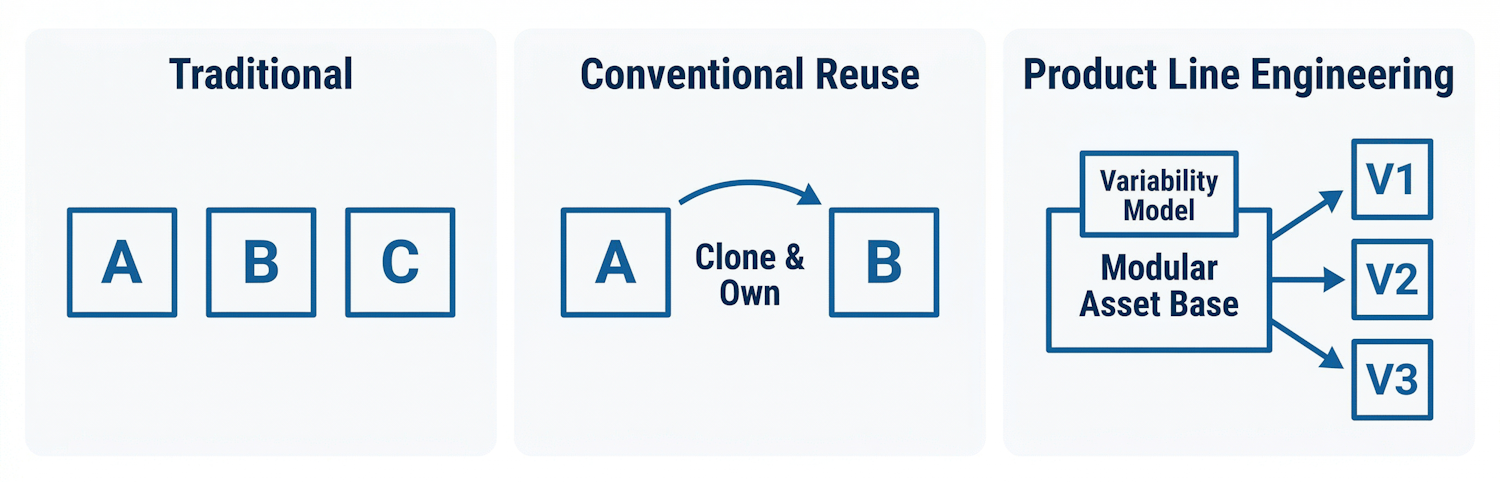
\includegraphics[width=\textwidth]{figures/placeholder_baukasten.png}
    \caption{Conceptual evolution from traditional product development to the Product Line Engineering (PLE) approach inspired by the "Baukasten" principle, illustrating the centralization of core assets.}
    \label{fig:baukasten_concept}
\end{figure}

This paper addresses the Agile Infrastructure Gap by introducing a formal three-tier architectural pattern for embedded variability management. Our approach, termed the Unified Variability Representation (UVR), collapses the traditional PLM stack into a single, portable LDraw file—the open standard for digital LEGO modeling. By leveraging LDraw's hierarchical referencing mechanism and a structured naming convention, we allow the 3D geometry to carry its own variability logic, making the model self-contained and machine-interpretable without the need for external mapping databases.

\section{Related Work}

The foundations of modern variability management were established by the SPLE community, with works by Pohl et al. \cite{Pohl2005} and Linden et al. \cite{Linden2007} defining the core processes of domain and application engineering. More recently, the emergence of the Universal Variability Language (UVL) \cite{Benavides2025UVL} has provided a standardized exchange format for feature models, facilitating tool interoperability in the problem space.

In the mechatronics and systems engineering domain, research has explored formalizing geometric constraints through SysML profiles \cite{warniez2014sysml} or integrating feature-based modeling with technical systems \cite{Koch2016}. While these approaches provide technical rigor, they often require specialized toolchains that remain disconnected from the immediate, visual 3D representation used by designers. Furthermore, as noted by Kuiter et al. \cite{KuiterTK25}, there is a growing need for modern pedagogical frameworks that make abstract variability concepts tangible for students.

Our work bridges these two worlds by providing a "geometric companion" to feature modeling. We build upon the open-source CADdrive platform \cite{Hackenberg2023}, which aims to provide GitHub-like collaboration for physical product design. By extending CADdrive with the UVR pattern, we demonstrate a low-barrier, high-rigor methodology for managing variant-rich systems that is equally suitable for agile industrial prototyping and mechatronic education. In the following sections, we formally define the UVR architecture and validate its application through a mechatronic drone case study.

\section{The Three-Tier Architecture for Embedded PLE}

The core contribution of this work is the formalization of a three-tier architectural pattern that enables the embedding of Product Lifecycle Management (PLM) stack capabilities directly within a standard CAD data structure. By applying the principle of **Separation of Concerns**, we organize the 150\% model into three functional layers, all contained within a single, traversable LDraw hierarchy. This modularity ensures that changes to the physical geometry do not inadvertently break the variability logic, and vice-versa.

\subsection{Architectural Layers}

As illustrated in Fig. \ref{fig:3_tier_arch}, the UVR hierarchy is organized into three primary branches, each serving a distinct role in the product line lifecycle:

\begin{enumerate}
    \item \textbf{Tier 1: Configurations (The Product Map):} This top-most layer defines the scope of the product line by listing the specific configurations currently offered. It is implemented using empty submodels (proxies) where the variant's name carries the selection logic. This layer acts as the "Sales Catalog" or "Product Map," identifying which combinations of features are officially supported as sellable variants.
    \item \textbf{Tier 2: Features (The Logical Model):} This layer implements the variability logic, acting as the bridge between the problem and solution spaces. It defines the hierarchical feature tree (e.g., Propeller $\rightarrow$ 2-Blade $\rightarrow$ Small) and encodes the logical constraints (XOR, OR, REQ, EXCL). Crucially, these logical nodes do not contain geometry themselves; instead, they **reference** the appropriate assets in Tier 3.
    \item \textbf{Tier 3: Parts (The Atomic Asset Base):} This foundation layer represents the "Baukasten" or physical asset base. it contains the atomic geometric definitions (e.g., a specific motor housing, a standardized M2 screw, or a custom carbon fiber arm). These components are strictly logic-free and are named descriptively. This separation allows mechatronic assets to be reused across multiple logical features without redundant definitions.
\end{enumerate}

\begin{figure}[bt]
    \centering
    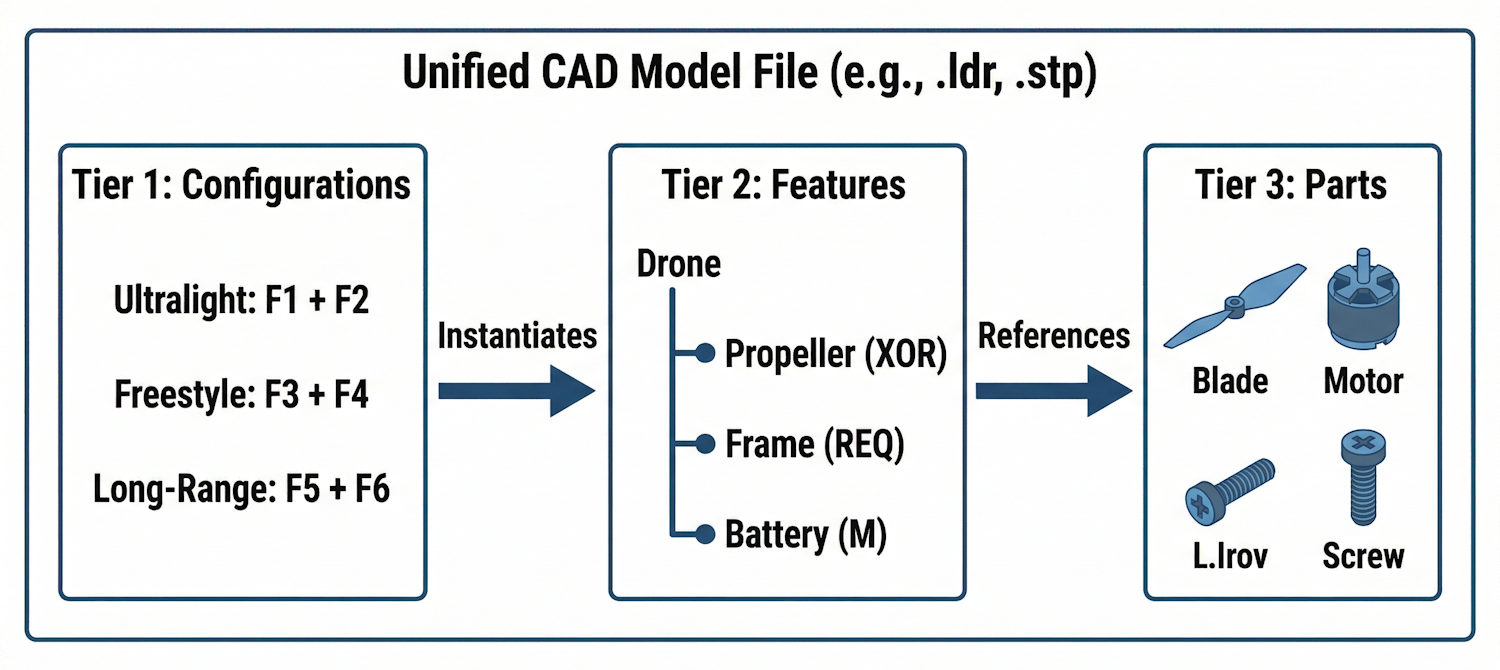
\includegraphics[width=\textwidth]{figures/placeholder_3_tier.png}
    \caption{The Three-Tier UVR Architecture: Separating product configurations from variability logic and physical assets within a single file hierarchy, ensuring a portable single source of truth.}
    \label{fig:3_tier_arch}
\end{figure}

\subsection{Formal Naming Convention}

To ensure that the 150\% model is "self-documenting" and machine-interpretable across any LDraw-compliant editor, UVR defines a systematic naming convention. This approach eliminates the need for proprietary plugins, as the variability metadata is preserved in the submodel definitions themselves. The convention is divided into four semantic categories:

\subsubsection{Feature Classification (Tier 2)}
These prefixes define the functional role of a node within the derivation tree:
\begin{itemize}
    \item \texttt{(M)} \textbf{Mandatory:} Indicates that the feature is a common asset and its resolved subtree must be included in every product variant.
    \item \texttt{(CF)} \textbf{Concrete Feature:} Identifies a selectable feature that directly maps to physical geometry or a specific mechatronic assembly in Tier 3.
    \item \texttt{(AF)} \textbf{Abstract Feature:} Defines a purely logical node used for hierarchical grouping (e.g., a group for all available battery sizes) without associated geometry.
\end{itemize}

\subsubsection{Group Logic (Tier 2)}
Applied to abstract features, these tags govern how child references must be resolved during configuration:
\begin{itemize}
    \item \texttt{(XOR)} \textbf{Exclusive OR:} Strictly one child feature must be selected (e.g., choosing exactly one frame size).
    \item \texttt{(OR)} \textbf{Inclusive OR:} At least one child feature must be selected, allowing for multi-selection where applicable.
\end{itemize}

\subsubsection{Cross-Tree Constraints (Tier 2)}
Suffixes are used to encode dependencies that violate the strict parent-child hierarchy, enabling the modeling of complex mechatronic interdependencies:
\begin{itemize}
    \item \texttt{(REQ: [Target])} \textbf{Requires:} Selection of the host feature programmatically forces the inclusion of the specified target feature.
    \item \texttt{(EXCL: [Target])} \textbf{Excludes:} Selection of the host feature prevents the inclusion of the target feature (e.g., preventing a Large Battery from being selected for a Small Frame).
\end{itemize}

\subsubsection{Configuration Formulas (Tier 1)}
Preconfigured variants are defined as empty submodels within the Configurations branch. The formula is embedded directly in the submodel name using a simple additive syntax that specifies the required concrete features:
\begin{center}
    \texttt{Variant\_Name ((CF) Feature\_A + (CF) Feature\_B + ...)}
\end{center}

\begin{figure}[bt]
    \centering
    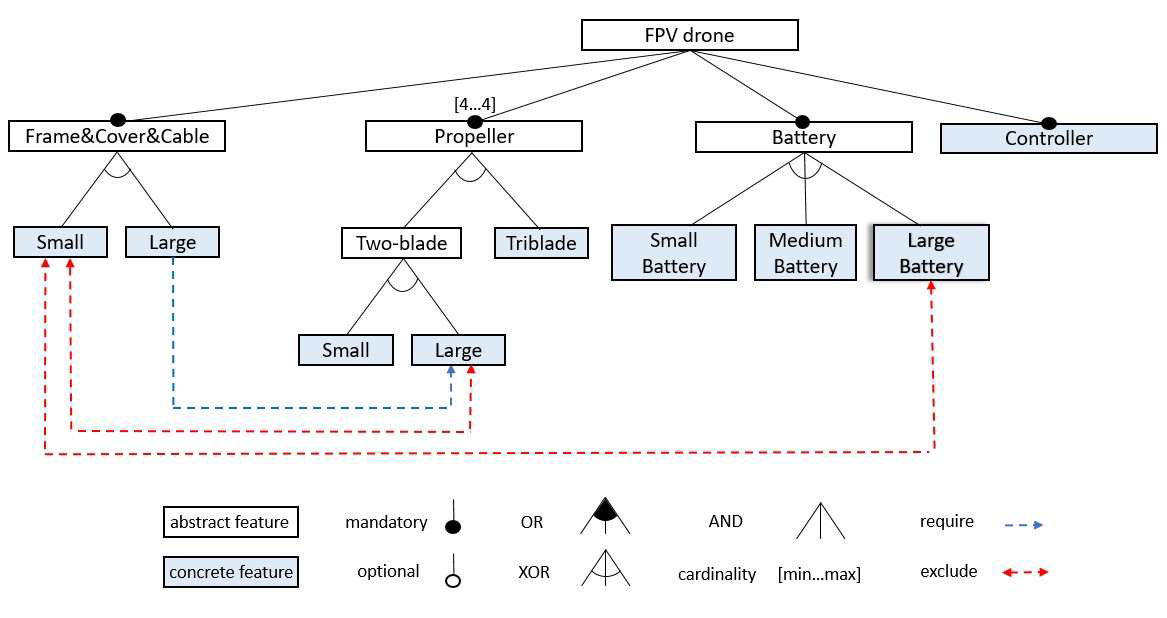
\includegraphics[width=0.9\textwidth]{figures/placeholder_feature_tree.png}
    \caption{Mapping of the naming convention to a graphical feature tree representation, demonstrating how the UVR nomenclature encodes the full logic of a variability model.}
    \label{fig:naming_convention}
\end{figure}

\subsection{Derivation Algorithm}

The derivation of a specific 3D product variant from the 150\% model follows a subtractive tree-filtering approach. This algorithm ensures that the generated model is both logically valid according to the feature model and physically consistent according to the geometric constraints. The process involves five key steps:

\begin{enumerate}
    \item \textbf{Parse Hierarchy:} The algorithm first parses the unified LDraw file to build an internal graph where nodes represent submodel definitions and edges represent their references (instantiations).
    \item \textbf{Retrieve Variant Formula:} Based on the user's requested variant name, the algorithm identifies the corresponding Tier 1 configuration submodel and extracts the selection formula from its name.
    \item \textbf{Resolve References:} Starting from the root, the algorithm recursively marks nodes as "Active." A node is activated if it is marked as Mandatory, if it is a Concrete Feature explicitly listed in the extracted formula, or if it is an essential abstract parent required to maintain the tree path.
    \item \textbf{Prune and Filter:} The algorithm traverses the graph and removes all non-active nodes and their entire subtrees. Any cross-tree constraints (\texttt{REQ/EXCL}) are validated at this stage to ensure the formula does not violate the underlying mechatronic rules.
    \item \textbf{Generate Output:} The final result is exported as a new, filtered LDraw file containing only the resolved physical components from Tier 3, positioned correctly in the world coordinate system.
\end{enumerate}

\section{Case Study: FPV Drone Product Line}

To validate the technical feasibility and architectural rigor of the UVR pattern, we applied it to a First-Person View (FPV) drone product line. FPV drones are highly suitable for mechatronic PLE research because they are inherently modular, yet exhibit severe performance trade-offs and geometric interdependencies. The choice of battery weight, propeller diameter, and frame stiffness directly affects the drone's flight dynamics and structural integrity.

\subsection{Constraint Identification}

A critical first step in mechatronic domain engineering is the systematic identification of physical constraints. Unlike software features, mechatronic modules occupy physical volumes and interact dynamically. Through spatial analysis within the digital LEGO environment, we identified two primary classes of constraints that our three-tier model must enforce:

\begin{enumerate}
    \item \textbf{Static Space Constraints:} These constraints arise from invariant geometric properties. For example, the central housing of our \textit{Small Frame} is designed for agility and weight reduction. Consequently, it has a strictly limited internal volume that can only accommodate the \textit{Small Battery} (450mAh). Attempting to mount a \textit{Large Battery} (1300mAh) results in a physical overlap, making the configuration unbuildable.
    \item \textbf{Dynamic Space Constraints:} These involve the operational envelopes of moving parts. While a \textit{Large Propeller} (5-inch) can be mounted onto the motors of a \textit{Small Frame} due to standardized hole patterns, the length of the propeller blades exceeds the distance to the frame's arms. During high-speed rotation, the blades would collide with the frame, leading to catastrophic failure. 
\end{enumerate}

\begin{figure}[bt]
    \centering
    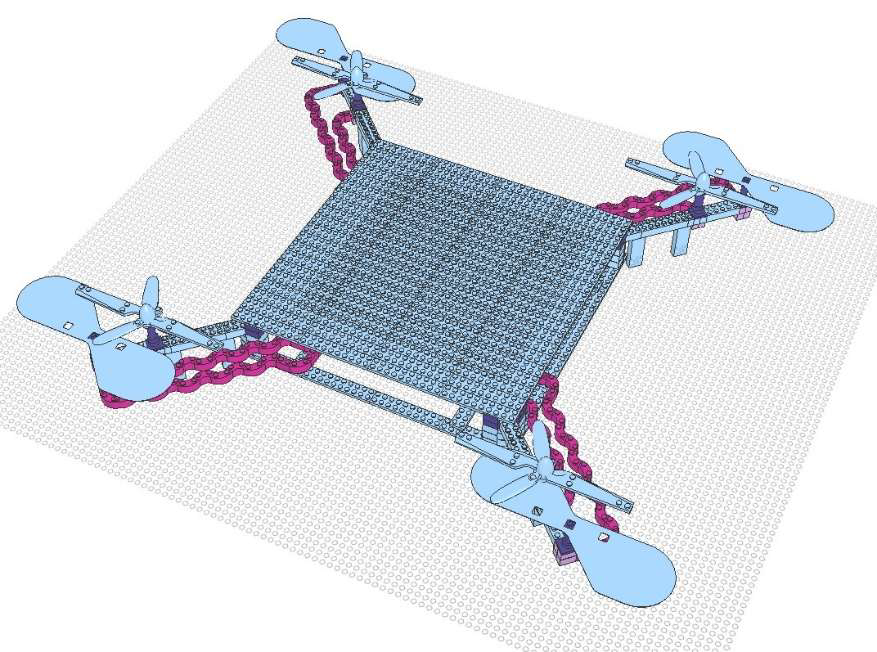
\includegraphics[width=0.9\textwidth]{figures/placeholder_150_model.png}
    \caption{The 150\% LDraw model of the FPV drone product line, showing the overlapping mechatronic modules in a single world coordinate system.}
    \label{fig:150_model}
\end{figure}

By formalizing these as \texttt{EXCL} and \texttt{REQ} constraints within the Tier 2 submodel names, we ensure that the derivation algorithm can prevent the generation of such invalid physical artifacts.

\subsection{Applying the 3-Tier Mapping}

The 150\% LDraw model for the drone product line is implemented as a single file where the root assembly instantiates the following hierarchical structure of submodel definitions:

\begin{itemize}
    \item \texttt{FPV\_Drone.ldr} (Root Assembly)
    \begin{itemize}
        \item \textbf{Configurations} (Abstract Group)
        \begin{itemize}
            \item \texttt{Ultralight\_Drone ((CF) Frame\_Small + (CF) Batt\_Small + ...).ldr}
            \item \texttt{Freestyle\_Drone ((CF) Frame\_Large + (CF) Batt\_Medium + ...).ldr}
            \item \texttt{Long-Range\_Drone ((CF) Frame\_Large + (CF) Batt\_Large + ...).ldr}
        \end{itemize}
        \item \textbf{Features} (Abstract Group)
        \begin{itemize}
            \item \texttt{(M\_CF) Controller.ldr} $\rightarrow$ References \texttt{FC\_Logic\_Board.ldr}
            \item \texttt{(M\_AF\_XOR) Battery\_Size.ldr}
            \begin{itemize}
                \item \texttt{(CF) Batt\_Small.ldr} $\rightarrow$ References \texttt{LiPo\_450mAh.ldr}
                \item \texttt{(CF) Batt\_Large.ldr} $\rightarrow$ References \texttt{LiPo\_1300mAh.ldr}
            \end{itemize}
            \item \texttt{(M\_AF\_XOR) Propeller\_Type.ldr}
            \begin{itemize}
                \item \texttt{(CF) Prop\_Small.ldr} $\rightarrow$ References \texttt{Blade\_2in.ldr}
                \item \texttt{(CF) Prop\_Large.ldr} $\rightarrow$ References \texttt{Blade\_5in.ldr}
            \end{itemize}
            \item \texttt{(M\_AF\_XOR) Frame\_Size.ldr}
            \begin{itemize}
                \item \texttt{(CF) Frame\_Small (EXCL: CF\_Batt\_Large).ldr} $\rightarrow$ Ref. \texttt{Arm\_Small.ldr}
                \item \texttt{(CF) Frame\_Large (REQ: CF\_Prop\_Large).ldr} $\rightarrow$ Ref. \texttt{Arm\_Large.ldr}
            \end{itemize}
        \end{itemize}
        \item \textbf{Parts} (Atomic Asset Base)
        \begin{itemize}
            \item \texttt{FC\_Logic\_Board.ldr} (LDraw Geometry)
            \item \texttt{LiPo\_450mAh.ldr} (LDraw Geometry)
            \item \texttt{Blade\_2in.ldr} (LDraw Geometry)
            \item \texttt{Arm\_Small.ldr} (LDraw Geometry)
            \item \texttt{M2\_Screw.ldr} (Reusable Asset)
        \end{itemize}
    \end{itemize}
\end{itemize}

This mapping illustrates the formal separation of concerns: Tier 1 handles variant selection, Tier 2 manages the variability logic and geometric constraints, and Tier 3 provides the reusable physical assets. Notably, Tier 2 features such as \texttt{Frame\_Small} reference both specific physical parts (e.g., \texttt{Arm\_Small}) and generic reusable parts like \texttt{M2\_Screw}, which is shared across the entire product line.

\subsection{Results: Derived Variants}

From the unified 150\% model, we successfully derived three distinct variants that represent the spectrum of the drone product line:
\begin{itemize}
    \item \textbf{Ultralight:} Utilizes the Small Frame and 450mAh battery. Optimized for weight and safety during indoor flight or educational exercises.
    \item \textbf{Freestyle:} Pairs the Large Frame with Medium Batteries and Triblade Propellers. Optimized for agility, thrust, and acrobatic flight.
    \item \textbf{Long-Range:} Utilizes the Large Frame and high-capacity 1300mAh battery. Optimized for efficiency and endurance during extended outdoor missions.
\end{itemize}

\begin{figure}[bt]
    \centering
    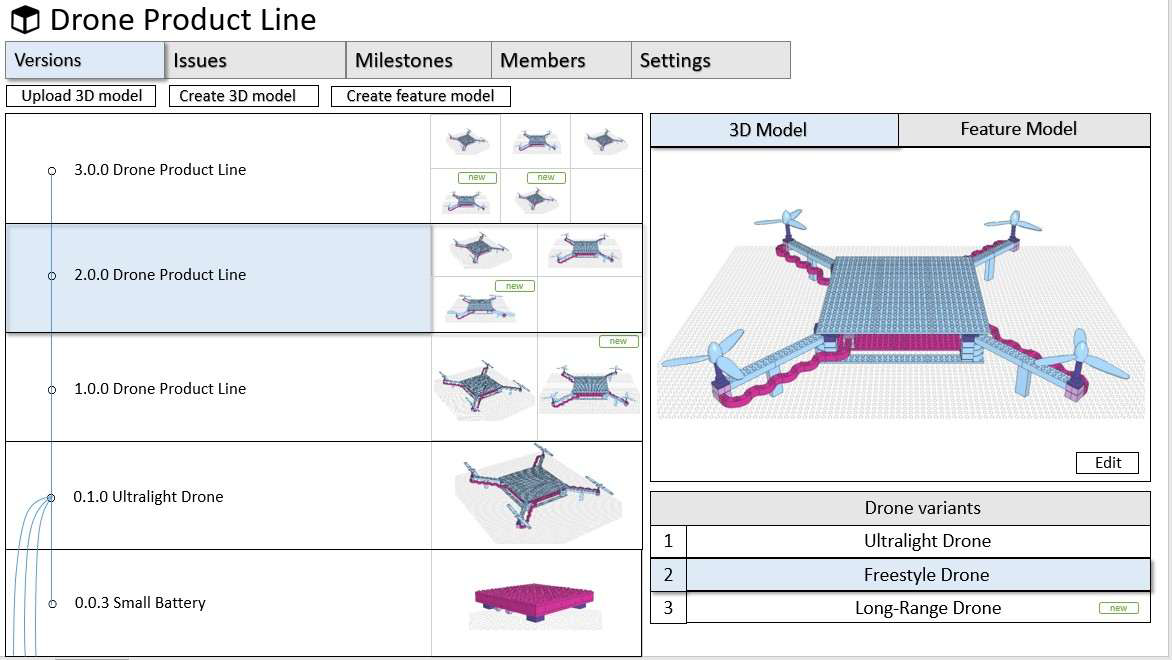
\includegraphics[width=0.9\textwidth]{figures/placeholder_variants.png}
    \caption{Three derived drone variants showcasing the subtractive filtering of the three-tier 150\% model, where each variant is logically and physically consistent.}
    \label{fig:derived_variants}
\end{figure}

The success of these derivations demonstrates that the UVR pattern effectively maintains the structural integrity of the mechatronic system while enabling rapid, automated product derivation. 

\section{Evaluation and Discussion}

The Three-Tier UVR pattern addresses the "Agile Infrastructure Gap" by providing a rigorous yet accessible methodology for early-phase mechatronic product line engineering. Our evaluation through the FPV drone case study reveals several key insights into the benefits and limitations of this approach.

\subsection{Structural Rigor and Scalability}

One of the most significant advantages of the three-tier separation is the decoupling of variability logic from physical geometry. By isolating atomic assets in Tier 3 (Parts), we ensure that the logical feature model in Tier 2 remains clean and maintainable. In traditional flat models, every geometric change (e.g., updating a screw size or motor mount) often requires a manual update of the configuration rules. In our pattern, a change to a Tier 3 submodel propagates automatically through the hierarchy. This structural rigor allows the product line to scale to hundreds of variants without the "configuration bloat" typically seen in early-phase mechatronic designs.

\subsection{Bridging the Pedagogical Barrier}

Beyond technical efficiency, the UVR pattern offers substantial educational value. By using digital LEGO as a "low-fidelity, high-rigor" proxy for mechatronic systems, we lower the barrier for students to experiment with complex PLE concepts. Students can visualize the impact of an \texttt{EXCL} constraint (e.g., propeller collisions) immediately in the 3D viewer, making abstract logical dependencies tangible. This hands-on experience aligns with modern pedagogical trends in systems engineering \cite{KuiterTK25} and provides a scalable alternative to costly industrial PLM training.

\subsection{Portability and the Research Ground Truth}

The reliance on standard LDraw submodel names and referencing hierarchies ensures that the UVR pattern is fully portable across different software environments. This is particularly relevant for the PLE research community, which often lacks shared, reproducible benchmarks for hardware-oriented variability. By providing a single-file "150\% ground truth" \cite{Strueber2019}, our approach enables researchers to test variant derivation and collision detection algorithms on a common, mechatronic artifact that does not require proprietary database access.

\section{Conclusion and Future Work}

This paper has presented the Three-Tier Unified Variability Representation (UVR), a novel architectural pattern for embedding variability management directly within mechatronic CAD models. By formally separating Configurations, Features, and Parts within a single, portable data structure, we bridge the "Agile Infrastructure Gap" between lightweight design and industrial-grade PLM. Our FPV drone case study demonstrates that this approach is both technically feasible and scientifically rigorous, providing a robust foundation for managing complex geometric and logical constraints.

Future research will focus on two primary directions. First, we aim to integrate the UVR naming convention with the emerging Universal Variability Language (UVL) standard \cite{Benavides2025UVL}, potentially creating a bidirectional bridge between 3D assets and standard problem-space models. Second, we plan to extend the pattern to manage multi-domain assets, such as firmware code and technical documentation, within the same hierarchical structure. Ultimately, we believe that embedding configuration intelligence directly into the geometry is a vital step toward making mechatronic product line engineering as agile and accessible as its software counterpart. 

\bibliographystyle{splncs04}
\bibliography{references}

\end{document}
